%%%%%%%%%%%%%%%%%%%%%%%%%%%%%%%%%%%%%%%%%%%
%%% DOCUMENT PREAMBLE %%%
\documentclass[12pt]{report}
\usepackage[italian]{babel}

\usepackage[normalem]{ulem}
\useunder{\uline}{\ul}{}
\usepackage{longtable}
\usepackage{url}
\usepackage{placeins}
\usepackage[utf8x]{inputenc}
\usepackage{amsmath}
\usepackage{graphicx}
\graphicspath{{images/}}
\usepackage{parskip}
\usepackage{fancyhdr}
\usepackage{vmargin}
\usepackage{nameref}
\setmarginsrb{3 cm}{2.5 cm}{3 cm}{2.5 cm}{1 cm}{1.5 cm}{1 cm}{1.5 cm}

\title{uCOM}								
% Title
\author{Mazzaglia Pietro}						
% Author

\makeatletter
\let\thetitle\@title
\let\theauthor\@author
\newcommand*{\currentname}{\@currentlabelname}
\makeatother

\pagestyle{fancy}
\fancyhf{}
\lhead{\thetitle}
\rhead{\currentname}
\cfoot{\thepage}


\begin{document}
	
	\huge \textbf{Elaborazione - Iterazione 4}
	
	\renewcommand{\thesection}{\arabic{section}}
	
	\normalsize
	
	%%%%%%%%%%%%%%%%%%%%%%%% PIANIFICAZIONE %%%%%%%%%%%%%%%%%%%%%%

	\section{Introduzione}
	
	Nota la seguente tabella di pianificazione:
	
	
	% Please add the following required packages to your document preamble:
	% \usepackage{graphicx}
	\begin{table}[!htb]
		\centering
		\resizebox{\textwidth}{!}{%
			\begin{tabular}{|l|l|l|}
				\hline
				\textbf{Priorità} & \textbf{Requisiti  (Casi d'uso o funzionalità)}                                                                          & \textbf{Commento}                                                                                                                                                                                                                                \\ \hline
				\textbf{Alta}              & \begin{tabular}[c]{@{}l@{}}\textbf{Invia comunicazione}\\ \\ \textbf{Invia avviso}\\ \\ \textbf{Gestisce utente}\\ \\ \textbf{Effettua accesso}\end{tabular} & \begin{tabular}[c]{@{}l@{}}\textbf{Nucleo della piattaforma, alta frequenza}\\ \\ \textbf{Nucleo della piattaforma, alta frequenza}\\ \\ \textbf{Nucleo della piattaforma, sicurezza}\\ \\ \textbf{Nucleo della piattaforma, sicurezza, coinvolta in tutte le funzioni}\end{tabular} \\ \hline
				\textbf{Media}             & \begin{tabular}[c]{@{}l@{}}\textbf{Prenota pasto}\\ \\ \textbf{Richiede libro}\end{tabular}                                                & \begin{tabular}[c]{@{}l@{}}\textbf{Frequenza elevata e più parti interessate ma sostituibile}\\ \\ \textbf{Frequenza elevata e più parti interessate ma sostituibile}\end{tabular}                                                                                 \\ \hline
				\textbf{Bassa}             & \begin{tabular}[c]{@{}l@{}}\textbf{Iscrive a un corso}\\ \\ \textbf{Gestisce corso}\\ \\ \textbf{Gestisce iscrizione corso}\end{tabular}            & \begin{tabular}[c]{@{}l@{}}\textbf{Bassa frequenza e sostituibile}\\ \\ \textbf{Bassa frequenza e sost5ituibile}\\ \\ \textbf{Bassa frequenza e sostituibile} \end{tabular}                                                                                                                                                \\ \hline
			\end{tabular}%
		}
	\end{table}
	
	Questa iterazione è l'ultima iterazione dell'elaborazione di uCOM, e non si occuperà di progettazione e implementazione di nuovi casi d'uso o scenari.
	
	Gli obiettivi della quarta iterazione sono:
	\begin{itemize}
		\item Analisi, relativamente ai casi d'uso \textit{UC3: Iscrive a un corso}, \textit{UC6: Gestisce iscrizione corso}
		\item Refactoring e e documentazione codice (laddove mancante) dell'iterazione 3
		\item Integrazione Database locale (MySQL) e ORM (\textit{Hibernate}) per il Registro Utenti utilizzato nel caso d'uso \textit{UC8: Gestisce utente}
	\end{itemize}
	
	
	\newpage
	
	\section{Modello dei casi d'uso}
	
	Seguono descrizioni dettagliate dei casi d'uso \textit{UC3} e \textit{UC6}.
	
	Inoltre si presentano i \textit{Diagrammi di sequenza di sistema} relativi agli scenari di successo.
	
	\subsection{UC3: Iscrive a un corso}

	% Please add the following required packages to your document preamble:
% \usepackage{longtable}
% Note: It may be necessary to compile the document several times to get a multi-page table to line up properly
\begin{longtable}{|l|l|}
	\hline
	\textbf{Nome caso d'uso} & UC3: Iscrive a un corso \\ \hline
	\endfirsthead
	%
	\endhead
	%
	\textbf{Portata} & Piattaforma uCOM \\ \hline
	\textbf{Livello} & Obiettivo utente \\ \hline
	\textbf{Attore primario} & Studente \\ \hline
	\textbf{\begin{tabular}[c]{@{}l@{}}Parti interessate \\ e Interessi\end{tabular}} & \begin{tabular}[c]{@{}l@{}}Studente: vuole iscriversi a un corso del Campus.\\ \\ Direzione Campus: vuole che i propri studenti possano\\ iscriversi ai corsi tramite la piattaforma fornita\end{tabular} \\ \hline
	\textbf{Pre-condizioni} & Lo Studente possiede un account sulla piattaforma. \\ \hline
	\textbf{Garanzia di successo} & Lo Studente ha ricevuto conferma dell'operazione. \\ \hline
	\textbf{\begin{tabular}[c]{@{}l@{}}Scenario principale \\ di successo\end{tabular}} & \begin{tabular}[c]{@{}l@{}}1. Lo Studente effettua l'accesso\\ 2. Lo Studente avvia l'operazione di iscrizione a un corso.\\ 3. Lo Studente indica il corso cui vuole iscriversi.\\ 4. Lo Studente invia l'iscrizione al corso.\\ 5. Il Sistema elabora l'iscrizione.\\ 6. Il Sistema conferma la riuscita dell'operazione.\end{tabular} \\ \hline
	\textbf{Estensioni} & \begin{tabular}[c]{@{}l@{}}*a. In qualsiasi momento.Il Sistema non è in grado di funzionare \\ correttamente in un dato momento.\\ \\     1) Il Sistema segnala l'impossibilità di eseguire l'azione.\\ \\     - Lo Studente riprova a eseguire l'azione dopo un certo periodo\\     di tempo.\\ \\ *b. In qualsiasi momento. Il Sistema entra in uno stato di errore\\ irrisolvibile.\\ \\     1) Il Sistema termina la sessione, perdendo i dati.\\ \\     - Lo Studente deve ricominciare l'operazione.\\ \\ *c. In qualsiasi momento. Lo Studente interrompe l'operazione.\\ \\ 1) Il Sistema termina l'operazione.\\ \\ 3a. Lo Studente indica un'opzione non valida o disponibile.\\ \\     1) Il Sistema richiede nuova immissione dei dati allo Studente.\\ \\ 5a. Lo studente non può iscriversi al corso selezionato.\\ \\   1a) Il Sistema indica il motivo per cui non è possibile iscriversi\\ e termina l'operazione.\end{tabular} \\ \hline
	\textbf{Requisiti speciali} & \begin{tabular}[c]{@{}l@{}}- Lo Studente deve inserire dati che siano conformi ai corsi\\ offerti dal Campus\end{tabular} \\ \hline
	\textbf{\begin{tabular}[c]{@{}l@{}}Elenco delle varianti \\ tecnologiche e dei dati\end{tabular}} & \begin{tabular}[c]{@{}l@{}}3) L'inserimento delle informazioni può avvenire attraverso\\ metodi input diversi, come tastiera e mouse o un touchscreen.\\ \\ 3) I Corsi disponibili sono quelli del Registro Corsi di uCOM.\end{tabular} \\ \hline
	\textbf{Frequenza di ripetizione} & bassa \\ \hline
	\textbf{Varie} & \begin{tabular}[c]{@{}l@{}}Si potrebbe prevedere un sistema che permetta l'inserimento\\ offline e l'elaborazione non appena il servizio ritorna disponibile.\\ \\ Si possono prevedere meccanismi di recupero dell'istanza in\\ caso di errori gravi.\end{tabular} \\ \hline
\end{longtable}	

	\newpage

	\subsection{UC6: Gestisce iscrizione corso}

	Questo caso d'uso è di tipo CRUD (Create Read Update Delete). Ai fini dello sviluppo di una versione di prova di \textit{uCOM} sarà trattato solo uno dei quattro scenari, ovvero quello di Creazione dell'iscrizione. Gli altri scenari saranno considerati come estensioni del caso d'uso.

	% Please add the following required packages to your document preamble:
% \usepackage[normalem]{ulem}
% \useunder{\uline}{\ul}{}
% \usepackage{longtable}
% Note: It may be necessary to compile the document several times to get a multi-page table to line up properly
\begin{longtable}{|l|l|}
	\hline
	\textbf{Nome caso d'uso} & UC6: Gestisce iscrizione corso \\ \hline
	\endfirsthead
	%
	\endhead
	%
	\textbf{Portata} & Piattaforma uCOM \\ \hline
	\textbf{Livello} & Obiettivo utente (CRUD) \\ \hline
	\textbf{Attore primario} & Amministratore \\ \hline
	\textbf{\begin{tabular}[c]{@{}l@{}}Parti interessate \\ e Interessi\end{tabular}} & \begin{tabular}[c]{@{}l@{}}Amministratore: vuole poter gestire la creazione di\\ un'iscrizione a un corso svolto internamente al Campus\\ \\ Direzione Campus: vuole che i corsi che si\\ svolgono all'interno del Campus siano gestite internamente dal\\ personale del Campus (Amministrazione)\end{tabular} \\ \hline
	\textbf{Pre-condizioni} & L'Amministratore possiede un account sulla piattaforma \\ \hline
	\textbf{Garanzia di successo} & \begin{tabular}[c]{@{}l@{}}Una nuova iscrizione è stata creata.\\ L'Amministratore ha ricevuto conferma dell'operazione.\end{tabular} \\ \hline
	\textbf{\begin{tabular}[c]{@{}l@{}}Scenario principale \\ di successo\end{tabular}} & \begin{tabular}[c]{@{}l@{}}1. L'Amministratore effettua l'accesso.\\ 2. L'Amministratore avvia l'iscrizione a un corso.\\ 3. L'Amministratore inserisce nome del corso e \\identificativo dello studente.\\ 4. L'Amministratore aggiunge l'iscrizione al Sistema.\\ 5. Il Sistema aggiunge l'iscrizione al proprio Registro Iscrizioni.\\ 6. Il Sistema conferma la riuscita dell'operazione.\end{tabular} \\ \hline
	\textbf{Estensioni} & \begin{tabular}[c]{@{}l@{}}*a. In qualsiasi momento.Il Sistema non è in grado di funzionare\\ correttamente in un dato momento.\\ \\ \quad1) Il Sistema segnala l’impossibilità a di eseguire l’azione. \\ \\ \quad- L'Amministratore riprova a eseguire l’azione dopo un certo \\ periodo di tempo.\\ \\ *b. In qualsiasi momento. Il Sistema entra in uno stato di errore \\ irrisolvibile. \\ \\ \quad1) Il Sistema termina la sessione, perdendo i dati. \\ \\ \quad- L'Amministratore deve ricominciare l’operazione.\\ \\ *c. In qualsiasi momento. L'Amministratore interrompe \\ l’operazione. \\ \\ \quad1) Il Sistema termina l’operazione.\\ \\ 2a. L'Amministratore avvia la lettura degli iscritti a un corso.\\ \\ \quad1) L'Amministratore inserisce il nome del Corso.\\ \\ \quad2) L'Amministratore richiede la lettura degli iscritti al corso.\\ \\ \quad3) Il Sistema preleva i dati relativi al corso richiesto \\ dal Registro Iscrizioni.\\ \\ \quad4) Il Sistema restituisce gli iscritti al corso richiesto.\end{tabular} \\ \hline
	\textbf{Estensioni} & \begin{tabular}[c]{@{}l@{}}2b. L'Amministratore avvia la modifica di un'iscrizione.\\ \\ \quad1) L'Amministratore inserisce le informazioni\\ relative a un'iscrizione da modificare.\\ \\ \quad2) L'Amministratore modifica l'iscrizione.\\ \\ \quad3) Il Sistema aggiorna l'iscrizione sul Registro Iscrizioni.\\ \\ \quad4) Il Sistema conferma la riuscita dell'operazione.\\ \\ 2c. L'Amministratore avvia l'eliminazione di un'iscrizione.\\ \\ \quad1) L'Amministratore inserisce le informazioni dell'iscrizione\\ da eliminare.\\ \\ \quad2) L'Amministratore elimina l'iscrizione.\\ \\ \quad3) Il Sistema elimina l'iscrizione dal Registro Iscrizioni.\\ \\ \quad4) Il Sistema conferma la riuscita dell'operazione.\\ \\ 3a. L'Amministratore inserisce informazioni non valide. \\ \\ \quad1) Il Sistema richiede nuova immissione dei dati \\ all'Amministratore\end{tabular} \\ \hline
	\textbf{Requisiti speciali} & Nessuno \\ \hline
	\textbf{\begin{tabular}[c]{@{}l@{}}Elenco delle varianti \\ tecnologiche e dei dati\end{tabular}} & \begin{tabular}[c]{@{}l@{}}3) L'inserimento delle informazioni può avvenire attraverso\\ metodi input diversi, come tastiera e mouse o un touchscreen.\\ \\ Le iscrizioni devono essere relative a\\ corsi esistenti nel Registro Corsi.\end{tabular} \\ \hline
	\textbf{Frequenza di ripetizione} & frequenza bassa \\ \hline
	\textbf{Varie} & \begin{tabular}[c]{@{}l@{}}Si potrebbero aggiungere nuove informazioni da memorizzare sul\\ Registro Iscrizioni.\end{tabular} \\ \hline
\end{longtable}	
	
	\newpage
	
	%%%%%%%%%%%%%% ANALISI ORIENTATA AGLI OGGETTI %%%%%%%%%%%%%%%%%
	
	\section{Modello di dominio}
	
	\subsection{Introduzione}
	
	Sulla base dei casi d'uso finora analizzati sono state identificate le seguenti classi concettuali:
	\begin{itemize}
		\item \textbf{Iscrizione}
		\item \textbf{Registro Iscrizioni}
	\end{itemize}

	Tenendo conto di associazioni e attributi, a partire dallo schema dell'Iterazione 1, è stato ricavato il seguente Modello di Dominio:
	
	\begin{center}	
	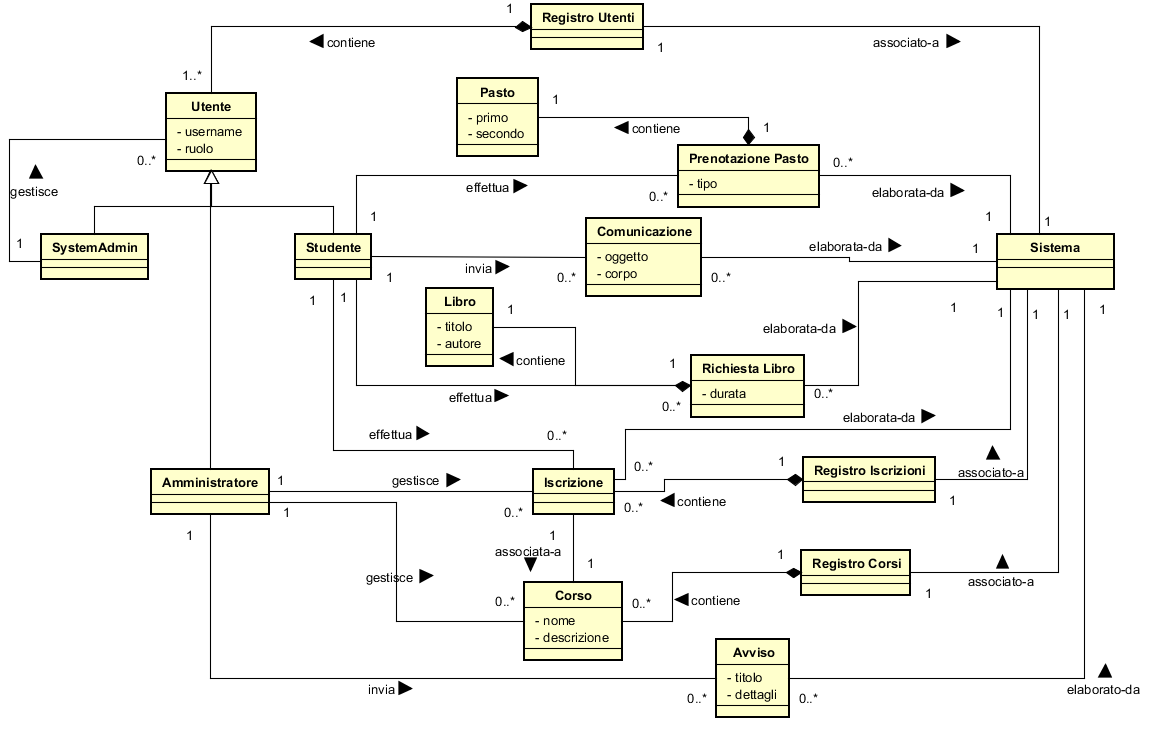
\includegraphics[scale=0.7]{./images/domain-I4.png}
	\end{center}
	
	I dettagli relativi alle classi sono stati inseriti nel \textbf{Glossario}.
	
	\newpage
	
	\section{Diagrammi di sequenza di sistema}
	
	I diagramma di sequenza di sistema mostrano gli eventi di I/O del sistema \textit{uCOM}, descrivendo in maniera chiara le interazioni tra attori e sistema.
	
	\subsection{UC3: Iscrive a un corso}
	\begin{center}
		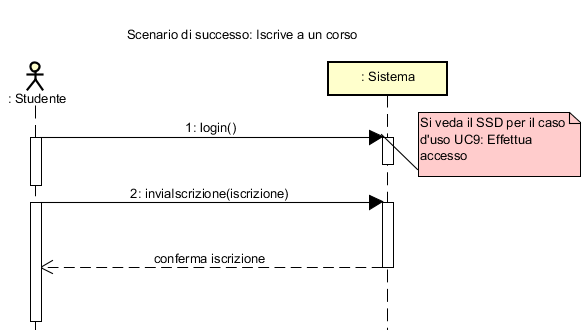
\includegraphics{./images/SSD_UC3.png}
	\end{center}
	
		
	\subsection{UC6: Gestisce iscrizione corso}
	
	\begin{center}
		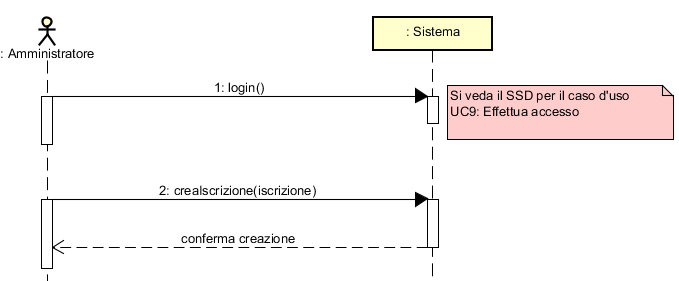
\includegraphics{./images/SSD_UC6.png}
	\end{center}
	
	
\end{document}